\chapter{Testing}
Testing is an important aspect of the work carried out in this thesis. In this chapter the
test setup are described. How the tests are carried out, some of the results and some
immediate results.


\section{Test Environment}
The test environment are two connected pipe segments. A Y-junction and an L-bend. This
pipe segments are connected, according to Figure \ref{chap7:fig-environment}.

\begin{figure}[htbp]
    \centering
    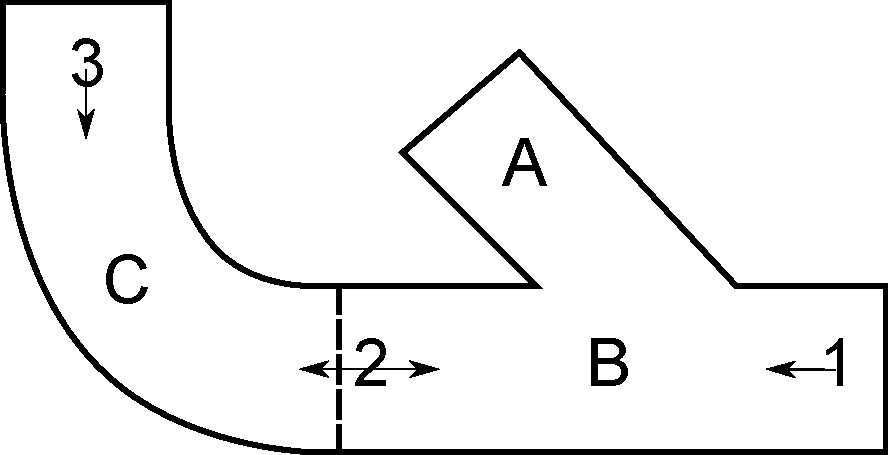
\includegraphics[width=0.7\textwidth]{pics/test-environment}
    \caption{The test environment}
    \label{chap7:fig-environment}
\end{figure}

There are six points of interest in this environment. 
The numbers 1-3 are the places where the sensors will be put and record snapshots of the pipe. 
The letters A-C are places where irregularities and anomalies in the pipes are placed. 

The idea behind the tests is to show how the sensors and the system reacts to different
kinds of anomalies, and how this impacts on the ability to detect what nodes is where. 


\section{Test Cases}
To test the performance and robustness of the developed algorithms three cases are used,
ideal situation, situation with obstacles with regular surface, and obstacles where the
surface are irregular. This cases are carried out for all the 3 different places described
in the previous section.

The tests are snapshots of the pipe at the given locations. This will test the abilities
of the system to recognize the environment and do the right decision. 


\subsection{Control/Ideal Case}
Here the sensors are placed at the different locations and the output are recorded. This
is for reference and what the data will look like in the ideal case. This should
considered perfect readings and all further readings will be measured up to this.


\subsection{Irregular surfaced anomalies}
The algorithm implemented relies greatly on regularity in the environment. The structure
of the surroundings are known to great extent and all irregularities and differences from
this are considered strange and are marked as anomalies. This case should test if this
works.

The tests are carried out with a curled-up paper which is placed at the three different
locations, marked in Figure \ref{chap7:fig-environment}. 
\begin{figure}[htbp]
    \centering
    \includegraphics[width=0.6\textwidth]{pics/curled-paper}
    \caption{The curled-up paper placed at point A in the pipe}
    \label{chap7:fig-culed-up-paper-at-A}
\end{figure}



\subsection{Regular surfaced anomalies}
As mentioned above the algorithm relies on regularity in the environment to detect
anomalies. This test will try to test the ability of the system to detect regular surfaced
objects which might look as they are a part of the environment. 

A stack of matchboxes are placed at the locations described and the data are recorded.
Figure \ref{chap7:fig-matchboxes-at-C} shows a picture of the stack of matchboxes placed
at Point C.
\begin{figure}[htbp]
    \centering
    \includegraphics[width=0.6\textwidth]{pics/matchboxesC}
    \caption{Stack of matchboxes placed at Point C}
    \label{chap7:fig-matchboxes-at-C}
\end{figure}



\section{Test Results}



